\subsection{Основные кинематические характеристики криволинейного движения: скорость и ускорение. Нормальное и тангенциальное ускорение}

\begin{definition}
    Траектория [S, м] - линия, вдоль которой движется тело.
\end{definition}

\begin{definition}
    Перемещение [$\Delta\vec{r}$, м] - направленный отрезок прямой, соединяющий начальное и последующее/конечное положения тела.
\end{definition}

\begin{definition}
    Путь [$S/l/S_{0}S_{end}$] - скалярная величина, равная длине участка траектории, по которой двигалось тело
\end{definition}

Рассмотрим участок траектории, который тело прошло за бесконечно малое время $(\Delta t\to0)$. 
Тогда и путь будет бесконечно малым, а значит, можно считать, что $\Delta S\to|\Delta\vec r|$, 
или же $\mathrm{d}s=|\mathrm{d}\vec r|$

\begin{figure}[h]
    \centering
    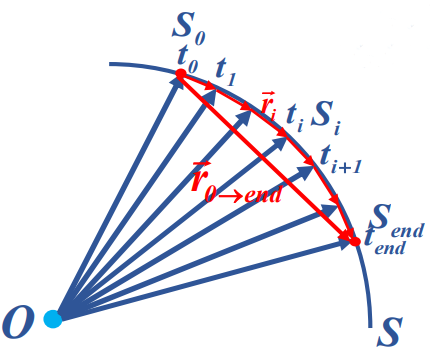
\includegraphics[width=0.5\linewidth]{imgs/q1i1.png}
    \caption{Вычисление пути и перемещения}
    \label{q1i1}
\end{figure}

\begin{definition}
    Полный путь тела — сумма всех суммарных (бесконечно малых) “подпутей”: $S_0S_{end}=\int\limits_{S_0}^{S_{end}}\mathrm{d}s=\int\limits_{S_0}^{S_{end}}|\mathrm{d}\vec r|$
\end{definition}

\begin{definition}
    Средняя скорость $[v_{ср}, \frac{м}{с}]$ — вектор, равный отношению перемещения ко времени пути: $v_{ср} = \frac{S}{t}$
\end{definition}

\begin{definition}
    Средняя путевая скорость $[v_{ср.п.}, \frac{м}{с}]$ — число, равное отношению пути ко времени в пути.
\end{definition}

\begin{definition}
    Мгновенная скорость  $[\vec v, \frac{м}{с}]$ — предел отношения перемещения ко времени на бесконечно малом промежутке времени: 
$\vec v = \lim\limits_{\Delta t\to0}\frac{\Delta\vec r}{\Delta t}$.
\end{definition}

\begin{definition}
    Скорость — векторная величина, характеризующая быстроту перемещения и направление движения материальной точки в пространстве относительно выбранной системы отсчёта
\end{definition}

\begin{definition}
    Ускорение $[\vec a, \frac{м}{с^2}]$ — векторная физическая величина, характеризующая быстроту изменения скорости тела.
\end{definition}

\begin{remark}
    Ускорение — быстрота изменения вектора скорости.
\end{remark}

$$d\vec v = \vec a(t) dt \implies \vec v(t) = \vec{v_0} + \int\limits_{t_0}^{t} \vec a(t) dt$$
$$\vec r(t) = \vec{r_0} + \int\limits_{t_0}^{t} \vec v(t)dt = \vec{r_0} + \vec{v_0}(t-t_0) + \int\limits_{t_0}^{t} dt \int\limits_{t_0}^{t} \vec a(t) dt$$

При равноускоренном движении
$$\vec\upsilon(t)=\vec{v_0}+\vec a(t-t_0)$$
$$\vec r(t)=\vec{t_0}+\vec{v_0}(t-t_0)+\frac{\vec a(t-t_0)^2}{2}$$


$$\vec{a} = \vec{v_t}' = \vec{r_t}''$$

$$\vec{v} = \vec{v_0} + \vec{a}t$$

$$\vec{r} = \vec{r_0} + \vec{v_0}t + \frac{\vec a t^2}{2}$$

$$\begin{cases}
a_x=\frac{\mathrm{d}\upsilon_x}{\mathrm{d}t}=\upsilon_x'=\frac{\mathrm{d}^2x}{\mathrm{d}t^2}=x''\\
a_y=\frac{\mathrm{d}\upsilon_y}{\mathrm{d}t}=\upsilon_y'=\frac{\mathrm{d}^2y}{\mathrm{d}t^2}=y''\\
a_z=\frac{\mathrm{d}\upsilon_z}{\mathrm{d}t}=\upsilon_z'=\frac{\mathrm{d}^2z}{\mathrm{d}t^2}=z''\\
\end{cases}$$

\begin{definition}
    Полное ускорение $a = \sqrt{a_\tau^2 + a_n^2}$    
\end{definition}

\begin{definition}
    Тангенциальное ускорение $[a_\tau, м/с^2]$ — численное значение изменения скорости.    
\end{definition}
 
\begin{remark}
    Тангенциальное ускорение — составляющая ускорения, которая направлена вдоль скорости. Описывает степень изменения скорости по модулю: $a_\tau = \frac{\Delta v}{\Delta t}$
\end{remark}

При равномерном движении по окружности, тангенциальное ускорение равно нулю. Если нужно записать в векторном виде, то сонаправлено единичному вектору.

\begin{definition}
    Центростремительное (нормальное) ускорение $[a_n]$ — составляющая ускорения тела, характеризующая быстроту изменения направления вектора скорости: $a_n=\frac{\upsilon^2}{r}$, где $r$ - радиус кривизны траектории в заданной точке.
\end{definition}

Центростремительное ускорение направлено к центру окружности, против вектора $\vec r$. 
Существует при движении по окружности, даже если линейная скорость константна, так как направление вектора скорости постоянно меняется.

\begin{figure}[h]
    \centering
    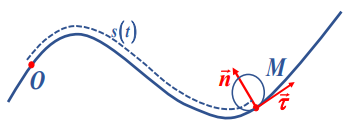
\includegraphics[width=0.5\linewidth]{imgs/q1i2.png}
    \label{q1i2}
\end{figure}

Вектор ускорения при движении по любой траектории можно записать как:

$$\vec a=a_\tau\vec\tau+a_n\vec n=\frac{d\upsilon}{dt}\vec\tau+\frac{\upsilon^2}{R}\vec n$$
$\vec\tau=\frac{\vec\upsilon}{|\vec\upsilon|}$ — единичный касательный к траектории вектор, направленный вдоль скорости;

$\vec n$ — единичный вектор, сонаправленный главной нормали к траектории.

